% Copyright 2007 by Till Tantau
%
% This file may be distributed and/or modified
%
% 1. under the LaTeX Project Public License and/or
% 2. under the GNU Public License.
%
% See the file doc/licenses/LICENSE for more details.



\documentclass{beamer}

%
% DO NOT USE THIS FILE AS A TEMPLATE FOR YOUR OWN TALKS�!!
%
% Use a file in the directory solutions instead.
% They are much better suited.
%


% Setup appearance:

\usetheme{Darmstadt}
\usefonttheme[onlylarge]{structurebold}
\setbeamerfont*{frametitle}{size=\normalsize,series=\bfseries}
\setbeamertemplate{navigation symbols}{}


% Standard packages

\usepackage[english]{babel}
\usepackage[latin1]{inputenc}
\usepackage{times}
\usepackage[T1]{fontenc}

% Setup TikZ
\usepackage{xcolor}
\usepackage{tikz}
\usetikzlibrary{arrows}
\tikzstyle{block}=[draw opacity=0.7,line width=1.4cm]


% Author, Title, etc.

\title[Distributed $3$D-Print Driver] 
{%
 Distributed \textbf{$3$}D-Print Driver
 %
}

\author[Guide]{
	\textbf{Presenter}: Suman~Bidarahalli \\
	\textbf{Supervisor}: \\
	Prof. Dr. Arjan~Kuijper \\  
	Alan~Brunton	\\ 
	Marco~Dennst{\"a}dt 
}
\institute[TU Darmstadt]
{
  Technische Universit�t Darmstadt, Germany
}

\date[ Master Thesis Presentation 2017]
{Master Thesis Presentation, February 2017}



% The main document

\begin{document}

\begin{frame}
  \titlepage
\end{frame}

\begin{frame}{Outline}
  \tableofcontents
\end{frame}


\section{Introduction}

\subsection{State of the art $3$D Print Driver}

\begin{frame}{Motivation}

\begin{columns}
    \begin{column}{0.25\textwidth}
    \centering
    \begin{figure}[!ht]
			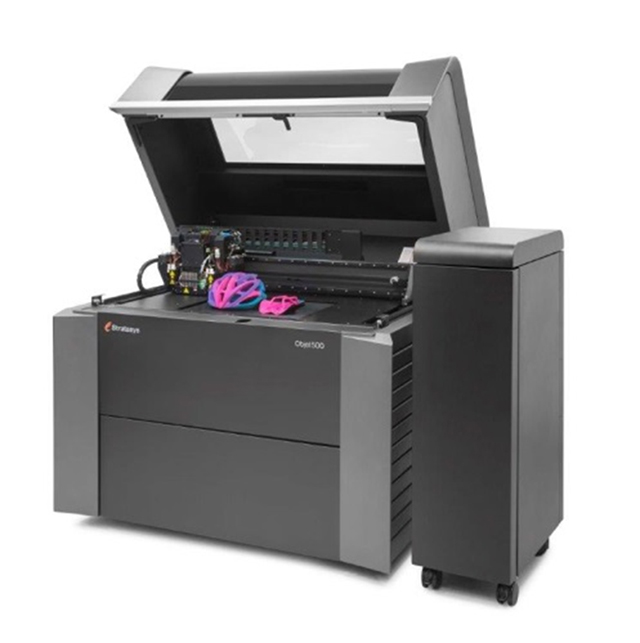
\includegraphics[width=0.90\textwidth]{PrinterI}
			\caption{State of the art $3$D Printers}
			\label{Fig:State of the art $3$D Printers}
		\end{figure}
    \end{column}
    \begin{column}{0.75\textwidth}
    \centering
    \begin{itemize}
			\item Today's $3$D Printers allow for multi-material high resolution prints
			\item Multiple objects in varying size can be printed at a go
			\item Voxel-level material assignment enables to reproduce high-fidelity appearance properties
			\item Larger print objects are composed of huge number of voxels
		\end{itemize} 
    \end{column}
  \end{columns}
\end{frame}

\subsection{Problem Statement}

\begin{frame}[t]{Requirement and Derived Goals}
\begin{columns}
    \begin{column}{0.45\textwidth}
    \centering
    \begin{figure}[!ht]
			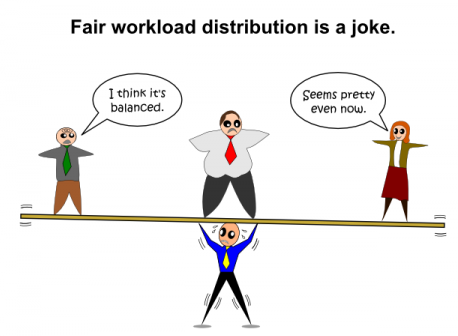
\includegraphics[width=0.90\textwidth]{SillyImage}
			\label{Fig:MythI}
		\end{figure}
    \end{column}
    \begin{column}{0.55\textwidth}
    \centering
    \begin{itemize}
    \item \textbf{Requirement}
		\begin{itemize}
		\item Provide Cuttlefish as cloud service
		\item Scaling of cluster nodes and fault tolerance
		\end{itemize} 
    \item \textbf{Derived Goals}
		\begin{itemize}
		\item Due application specific limitations, changed to cluster computing
		\item Creating a distributed version of cuttlefish with an abstraction layer 
		\end{itemize} 
		\end{itemize} 
    \end{column}
  \end{columns}
\end{frame}

\section{Solution}

%\subsection{What is a Distributed system? }
%\begin{frame} {Infrastructure for distribution}
%\begin{columns}
  %\begin{column}{0.50\textwidth}
  %\centering
	%\begin{figure}[!ht]
			%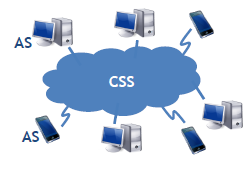
\includegraphics[width=0.90\textwidth]{DistributeIII.PNG}
			%\caption{Distributed System}
			%\label{Fig:DS}
		%\end{figure}
	%\end{column}
	%\begin{column}{0.50\textwidth}
		 %A \textbf{\textit{Distributed System}} is a cluster of AS where in each AS is connected to other by a network and primarily communicate via message passing
	%\end{column}
%\end{columns}
%\end{frame}

\begin{frame}{Currently used Distributed System}
\begin{columns}
  \begin{column}{0.50\textwidth}
  \centering
    \begin{figure}[!ht]
			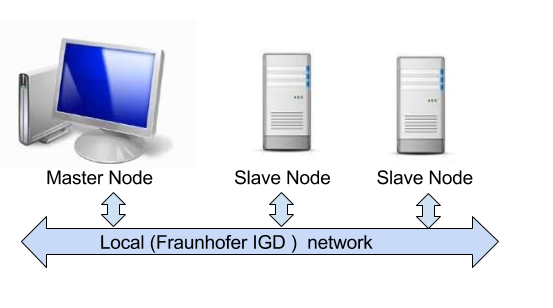
\includegraphics[width=0.90\textwidth]{ArchitectureI.png}
			\caption{Distributed System Architecture}
			\label{Fig:DCArchitecture}
		\end{figure}
	\end{column}
	\begin{column}{0.50\textwidth}
	\begin{itemize}
	\item The distributed system used is a cluster of heterogeneous systems 
	\item The nodes are connected via local(Fraunhofer) network
	\item All the nodes also have access to a shared network file system
	\end{itemize}	
	\end{column}
\end{columns}
\end{frame}

\begin{frame}{Master-Slave Paradigm}
\begin{columns}
  \begin{column}{0.30\textwidth}
  \centering
    \begin{figure}[!ht]
			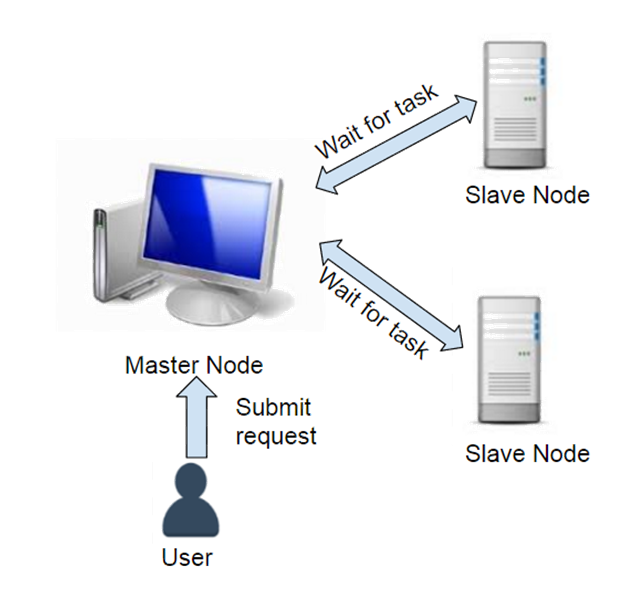
\includegraphics[width=0.90\textwidth]{TaskSubmission.PNG}
			\caption{Step 1:Task Submission}
			\label{Fig:TaskSubmission}
		\end{figure}
	\end{column}
	\begin{column}{0.30\textwidth}
		\begin{figure}[!ht]
			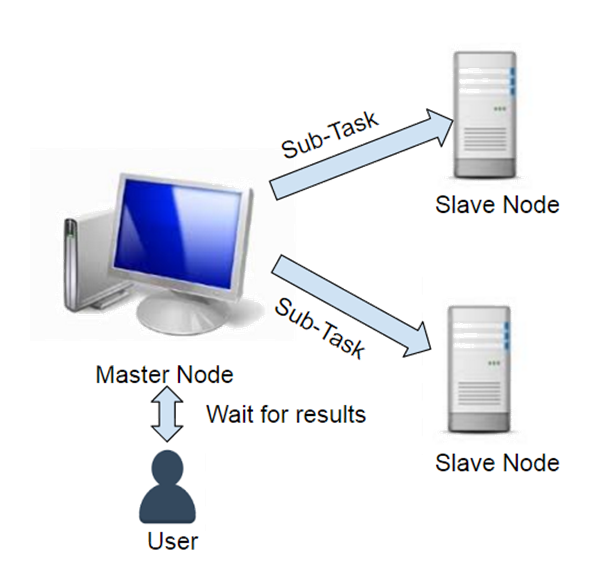
\includegraphics[width=0.90\textwidth]{TaskDistribution.PNG}
			\caption{Step 2: Sub-Task Computation}
			\label{Fig:TaskDistribution}
		\end{figure}
	\end{column}
		\begin{column}{0.30\textwidth}
		\begin{figure}[!ht]
			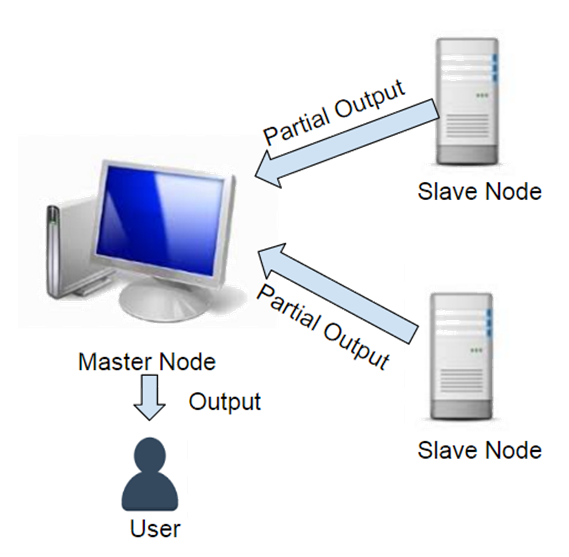
\includegraphics[width=0.90\textwidth]{CollectionAndMerging.PNG}
			\caption{Step 3: Partial Result Collection and Merging}
			\label{Fig:CollectionAndMerging}
		\end{figure}
	\end{column}
\end{columns}
\end{frame}

%\begin{frame}{Sub-Task Computation \& Partial Results Reporting}
%\begin{columns}
  %\begin{column}{0.50\textwidth}
  %\centering
    %\begin{figure}[!ht]
			%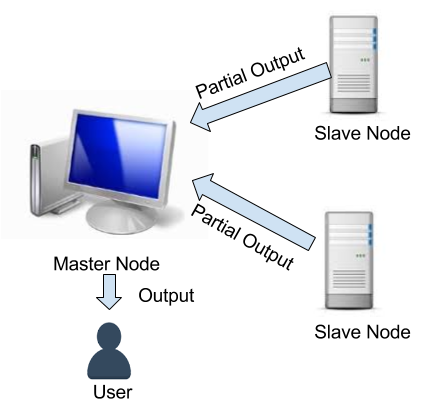
\includegraphics[width=0.90\textwidth]{ArchitectureIII}
			%\caption{Sub-Task Computation}
			%\label{Fig:ArchitectureIII}
		%\end{figure}
	%\end{column}
	%\begin{column}{0.50\textwidth}
	%\begin{itemize}
	%\item The slave nodes perform the computation locally
	%\item The output of the computation performed by the slaves is then reported back to the master node
	%\item The master node performs final computation using the received partial output from the slaves to provide the user with the final output
	%\end{itemize}	
	%\end{column}
%\end{columns}
%\end{frame}

\subsection{How is the distribution done?}
\begin{frame}{Different possibilities of distribution}
\begin{columns}
   \begin{column}{0.50\textwidth}
    \centering
    \begin{figure}[!ht]
			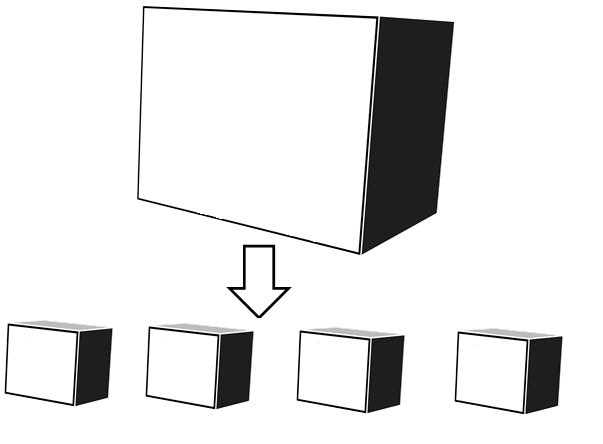
\includegraphics[width=0.90\textwidth]{DistributeI}
			\caption{Distribution of one large print object amongst the workstations }
			\label{Fig:DistributeI}
		\end{figure}
   \end{column}
	\begin{column}{0.50\textwidth}
    \centering
    %\begin{itemize}
		 %\item Distribution of one large print object amongst the workstations 
		 %\item Distribution of multiple print objects amongst the workstations
		 %\end{itemize} 
			\begin{figure}[!ht]
			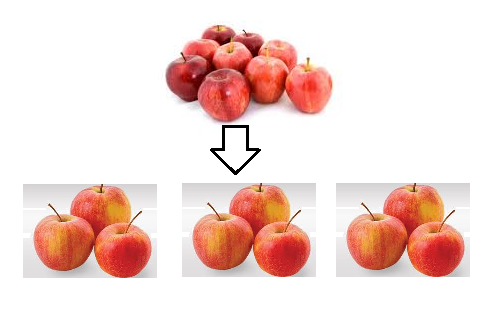
\includegraphics[width=0.90\textwidth]{DistributeII}
			\caption{Distribution of multiple print objects amongst the workstations}
			\label{Fig:DistributeII}
		\end{figure}
    \end{column}
  \end{columns}
  \end{frame}
	
\begin{frame}{Distribution of Sub-Tasks Using Cost Function}
\begin{itemize}
	\item For each object \textit{i}, compute volume
	\item Volume of the object \begin{math}V^i= w*h*l\end{math}
	\item Total Volume(k objects)=\begin{math}\sum\limits_{i=1}^{k}{V^i}\end{math}
	\item Threshold (for cluster size n-1)=\begin{math}(\sum\limits_{i=1}^{k}{V^i})/(n-1)\end{math}
\end{itemize}
\end{frame}	

%\begin{frame}{Chosen distribution}
    %\begin{itemize}
		%\item Multiple print objects will be distributed amongst the workstations i.e. each workstation performs computation on one or more whole inputs
		%\item The distribution of the workload and the collection of partial results is done through MPI(Message Passing Interface)
		%\end{itemize}
%\end{frame}

\subsection{Distributed Cuttlefish Application}
\begin{frame}{Current Component Architecture}
\begin{block}{Streaming Architecture}
	\begin{figure}[!ht]
		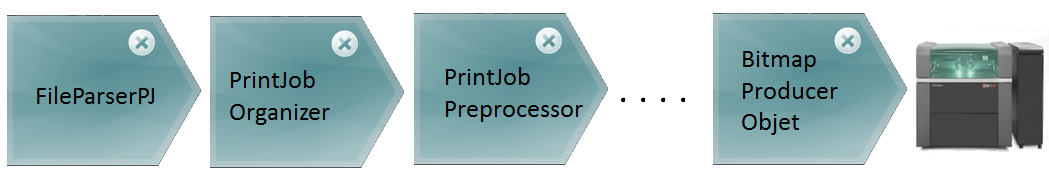
\includegraphics[width=0.9\textwidth]{StreamingArchitectureI.PNG}
		\caption{Cuttlefish Streaming Architecture}
		\label{Fig:CuttlefishPipelineFigure}
	\end{figure}
\end{block}
		%\item Cuttlefish Streaming architecture enables to perform the computation serially in a chunk-wise manner for each print object 
	\textbf{Goal}: To \textbf{retain the architecture} and is achieved by providing distinguished components to handle
	\begin{itemize} 
	\item  Distribution of sub-tasks 
	\item  Distribution of partial results
	\item  Collection of the partial results
	\end{itemize} 
\end{frame}


\begin{frame}{Classification of Prototypes}
\begin{block}{Distributed Cuttlefish Prototypes}
	\begin{figure}[!ht]
		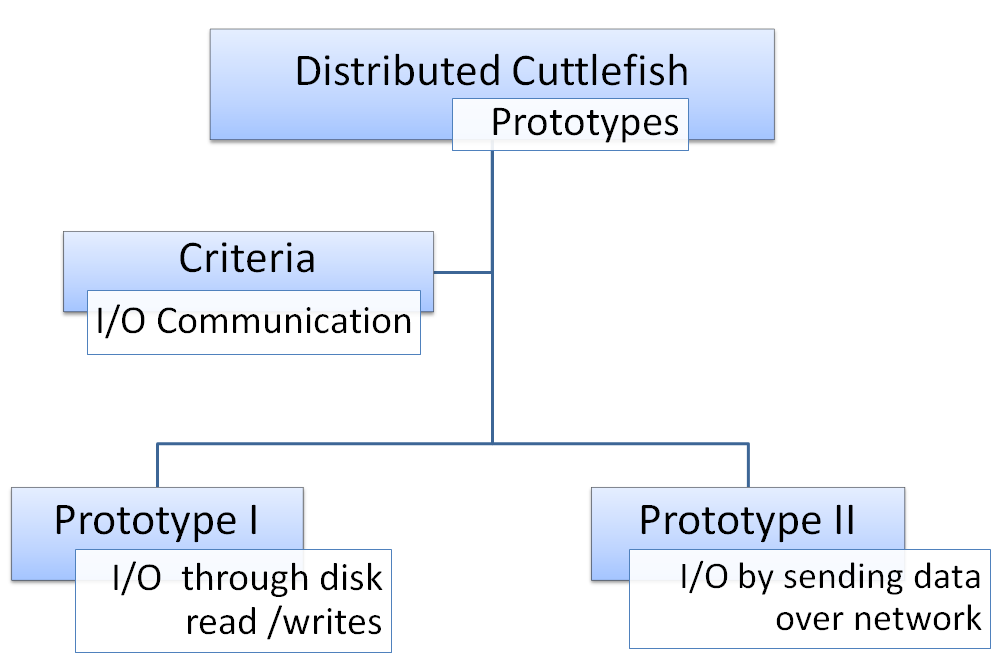
\includegraphics[width=0.9\textwidth]{Prototypes.PNG}
		\label{Fig:StreamingArchitectureI}
	\end{figure}
\end{block}
\end{frame}

\begin{frame}{Modified Component Architecture- Prototype I}
\begin{block}{Master Printing Software }
	\begin{figure}[!ht]
		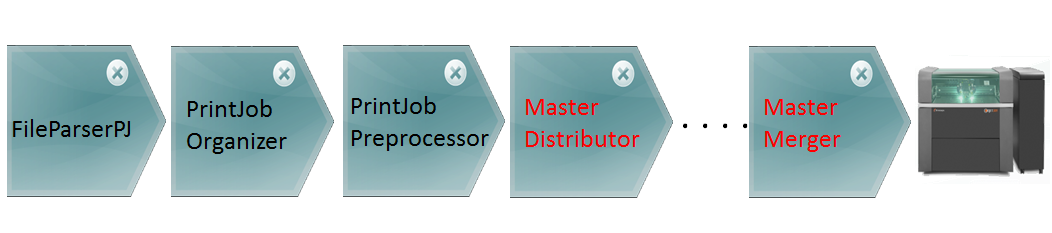
\includegraphics[width=0.9\textwidth]{MSPSPI.png}
		\label{Fig:MasterPSPl}
	\end{figure}
\end{block}
	\begin{block}{Slave Printing Software }
	\begin{figure}[!ht]
		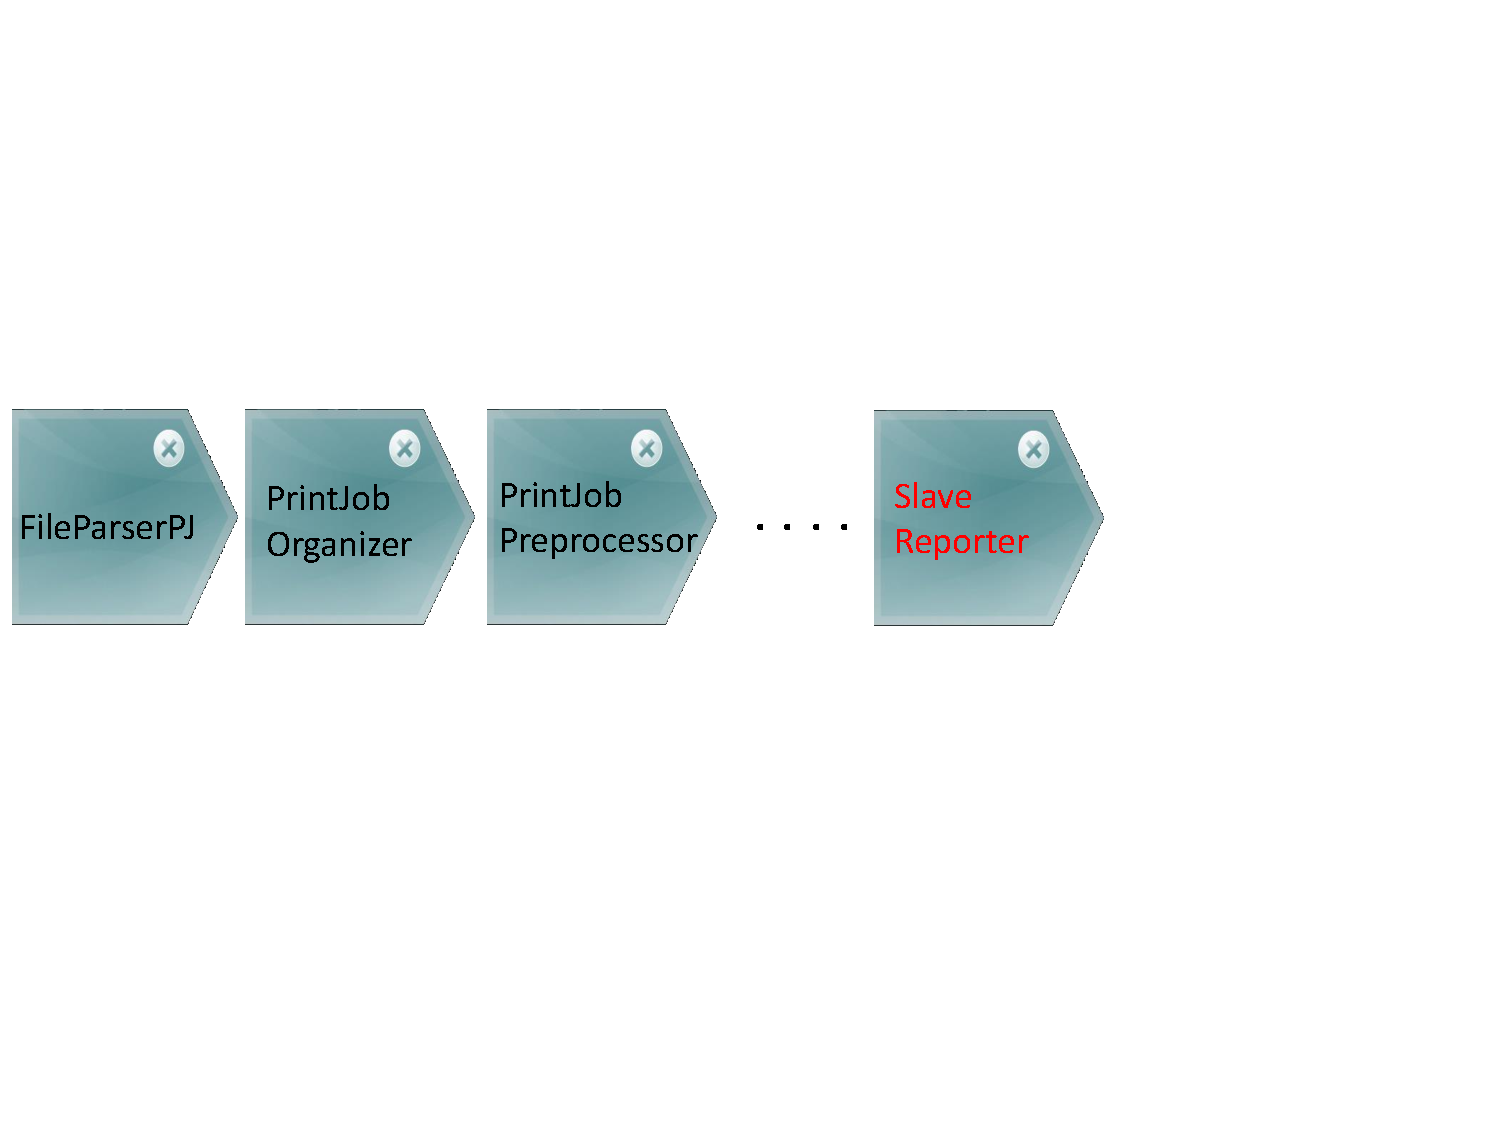
\includegraphics[width=0.8\textwidth]{SlavePSPI.png}
		\label{Fig:SlavePSPI}
	\end{figure}
\end{block}
\end{frame}

\begin{frame}{Modified Component Architecture- Prototype II}
\begin{block}{Master Printing Software }
	\begin{figure}[!ht]
		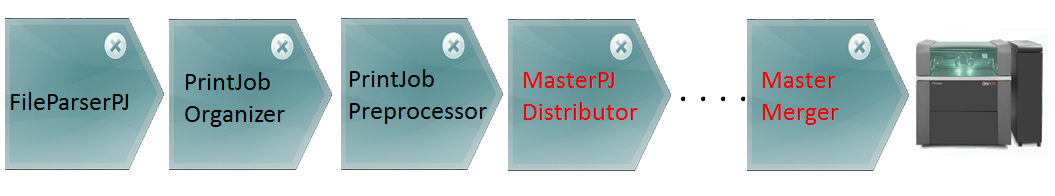
\includegraphics[width=0.9\textwidth]{MSPSPII.png}
		\label{Fig:MasterPSPIl}
	\end{figure}
\end{block}
	\begin{block}{Slave Printing Software }
	\begin{figure}[!ht]
		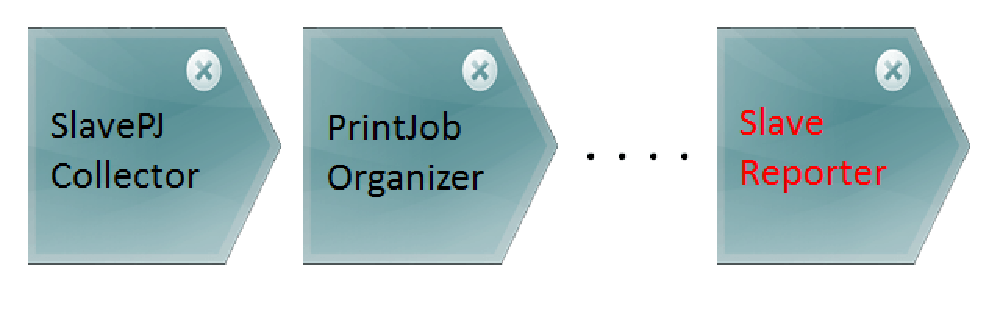
\includegraphics[width=0.8\textwidth]{SlavePSPII.png}
		\label{Fig:SlavePSPII}
	\end{figure}
\end{block}
\end{frame}

%\begin{frame}{Producer-Consumer}
	%\begin{figure}
		%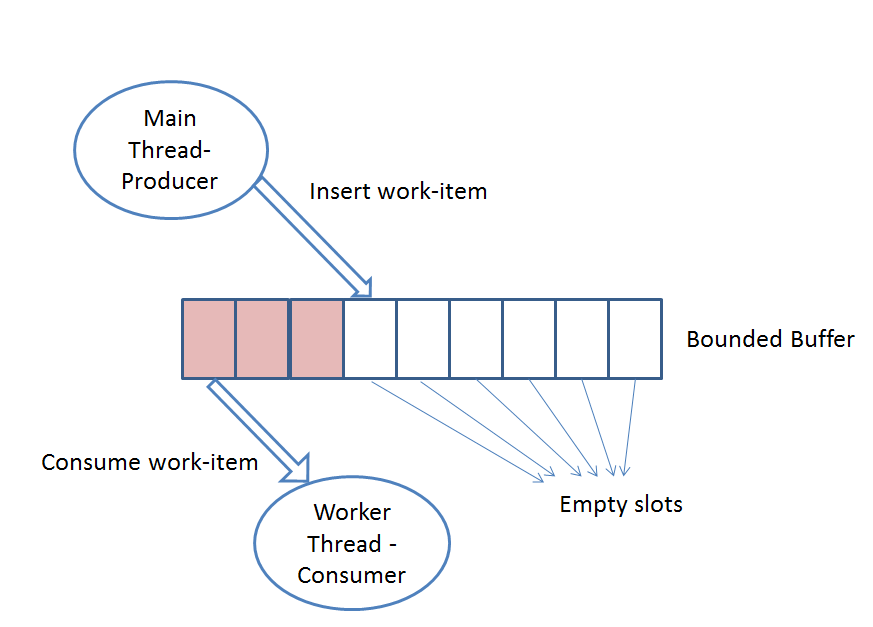
\includegraphics[width=0.9\textwidth]{ProducerConsumer.PNG}
	%\end{figure}	
%\end{frame}
\begin{frame}{Abstraction Layer}
	\begin{figure}
		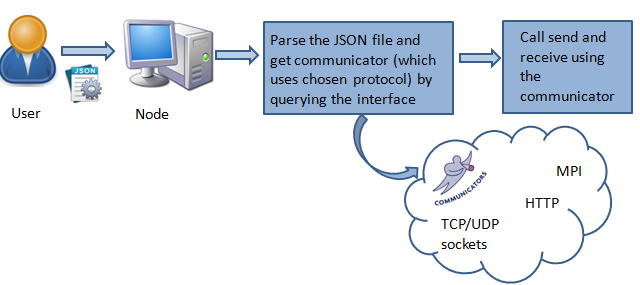
\includegraphics[width=0.9\textwidth]{AbstractionLayer.PNG}
	\end{figure}	
\end{frame}

\begin{frame}{Slave Reporter Component}
	\begin{figure}
		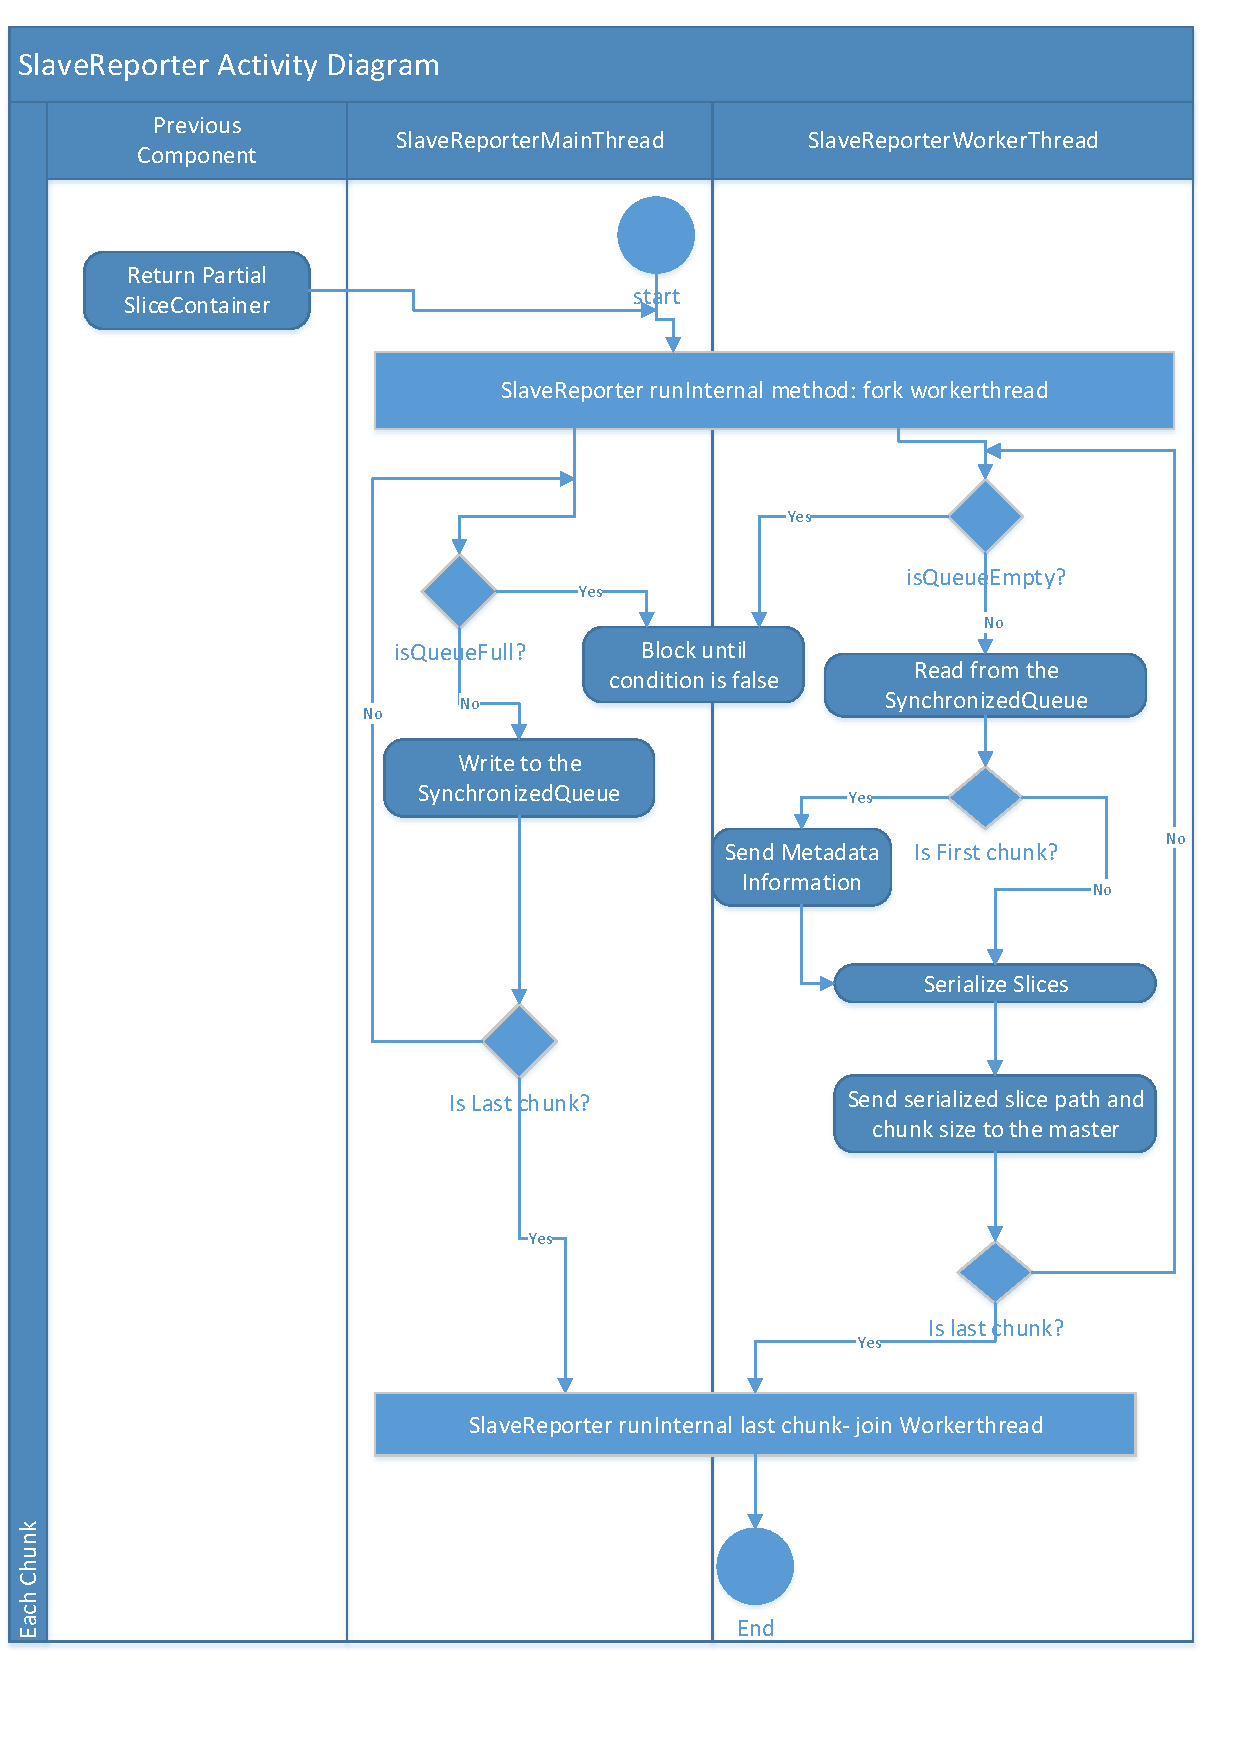
\includegraphics[width=0.50\textwidth]{SlaveReporter.pdf}
		\label{Fig:SlaveReporter}
	\end{figure}	
\end{frame}

\begin{frame}{Master Merger Component}
	\begin{figure}
		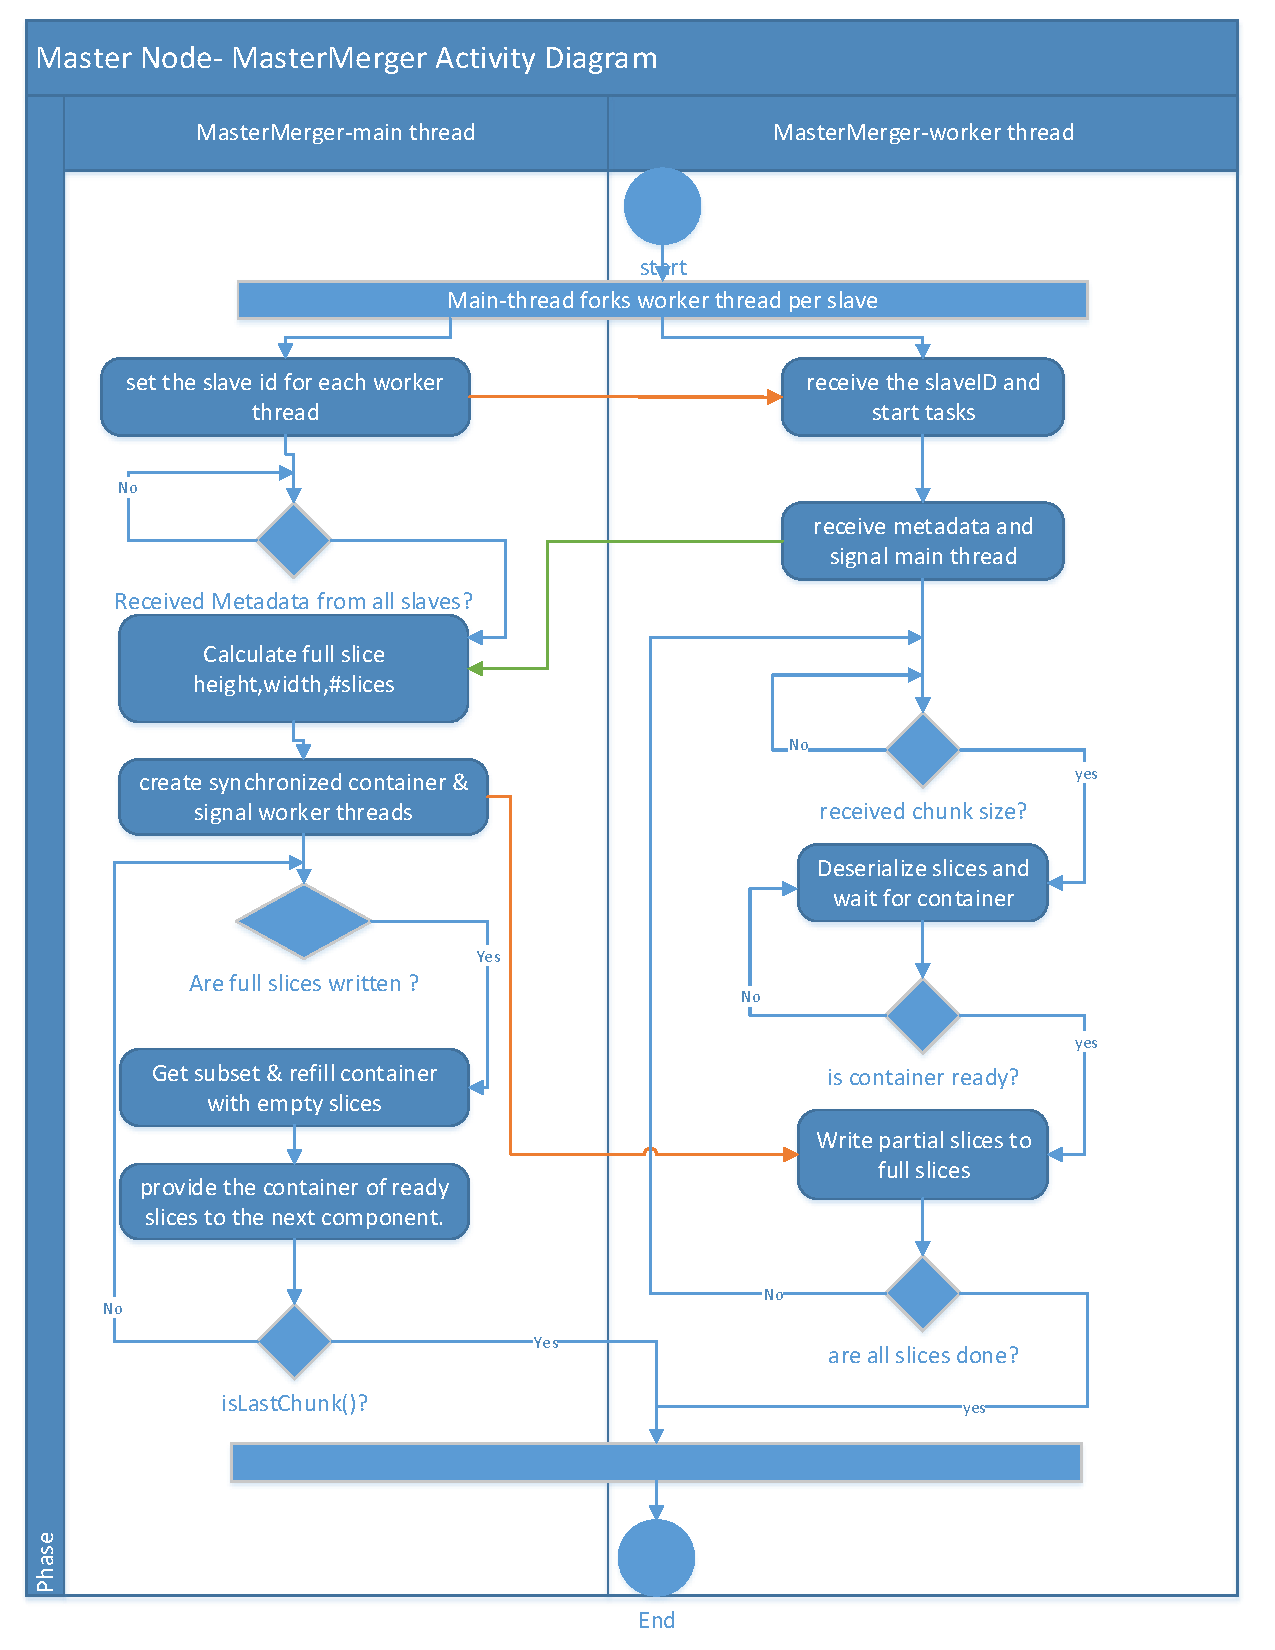
\includegraphics[width=0.55\textwidth]{MasterMerger.pdf}
		\label{Fig:MasterMerger}
	\end{figure}	
\end{frame}

\begin{frame}{Distributed Computing Tasks}
\begin{block}{Serialization And Deserialization}
	\begin{figure}[!ht]
		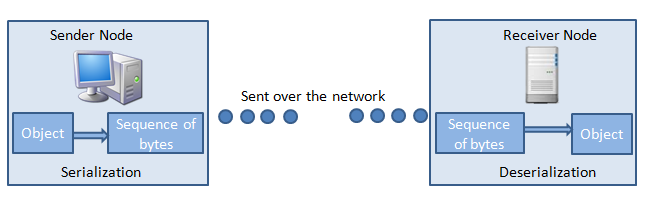
\includegraphics[width=0.7\textwidth]{Ser-Deser.PNG}
		\label{Fig:Ser-Deser}
	\end{figure}
\end{block}
	\begin{block}{Compression And Decompression}
	\begin{figure}[!ht]
		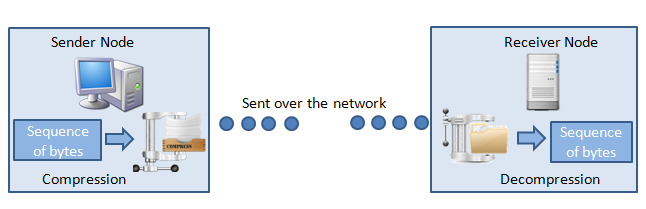
\includegraphics[width=0.7\textwidth]{CompDecomp.PNG}
		\label{Fig:CompDecomp}
	\end{figure}
\end{block}
\end{frame}

\section{Results}
\subsection{Distributed Cuttlefish vs Non-Distributed Cuttlefish}
\begin{frame}
\begin{figure}[!ht]
		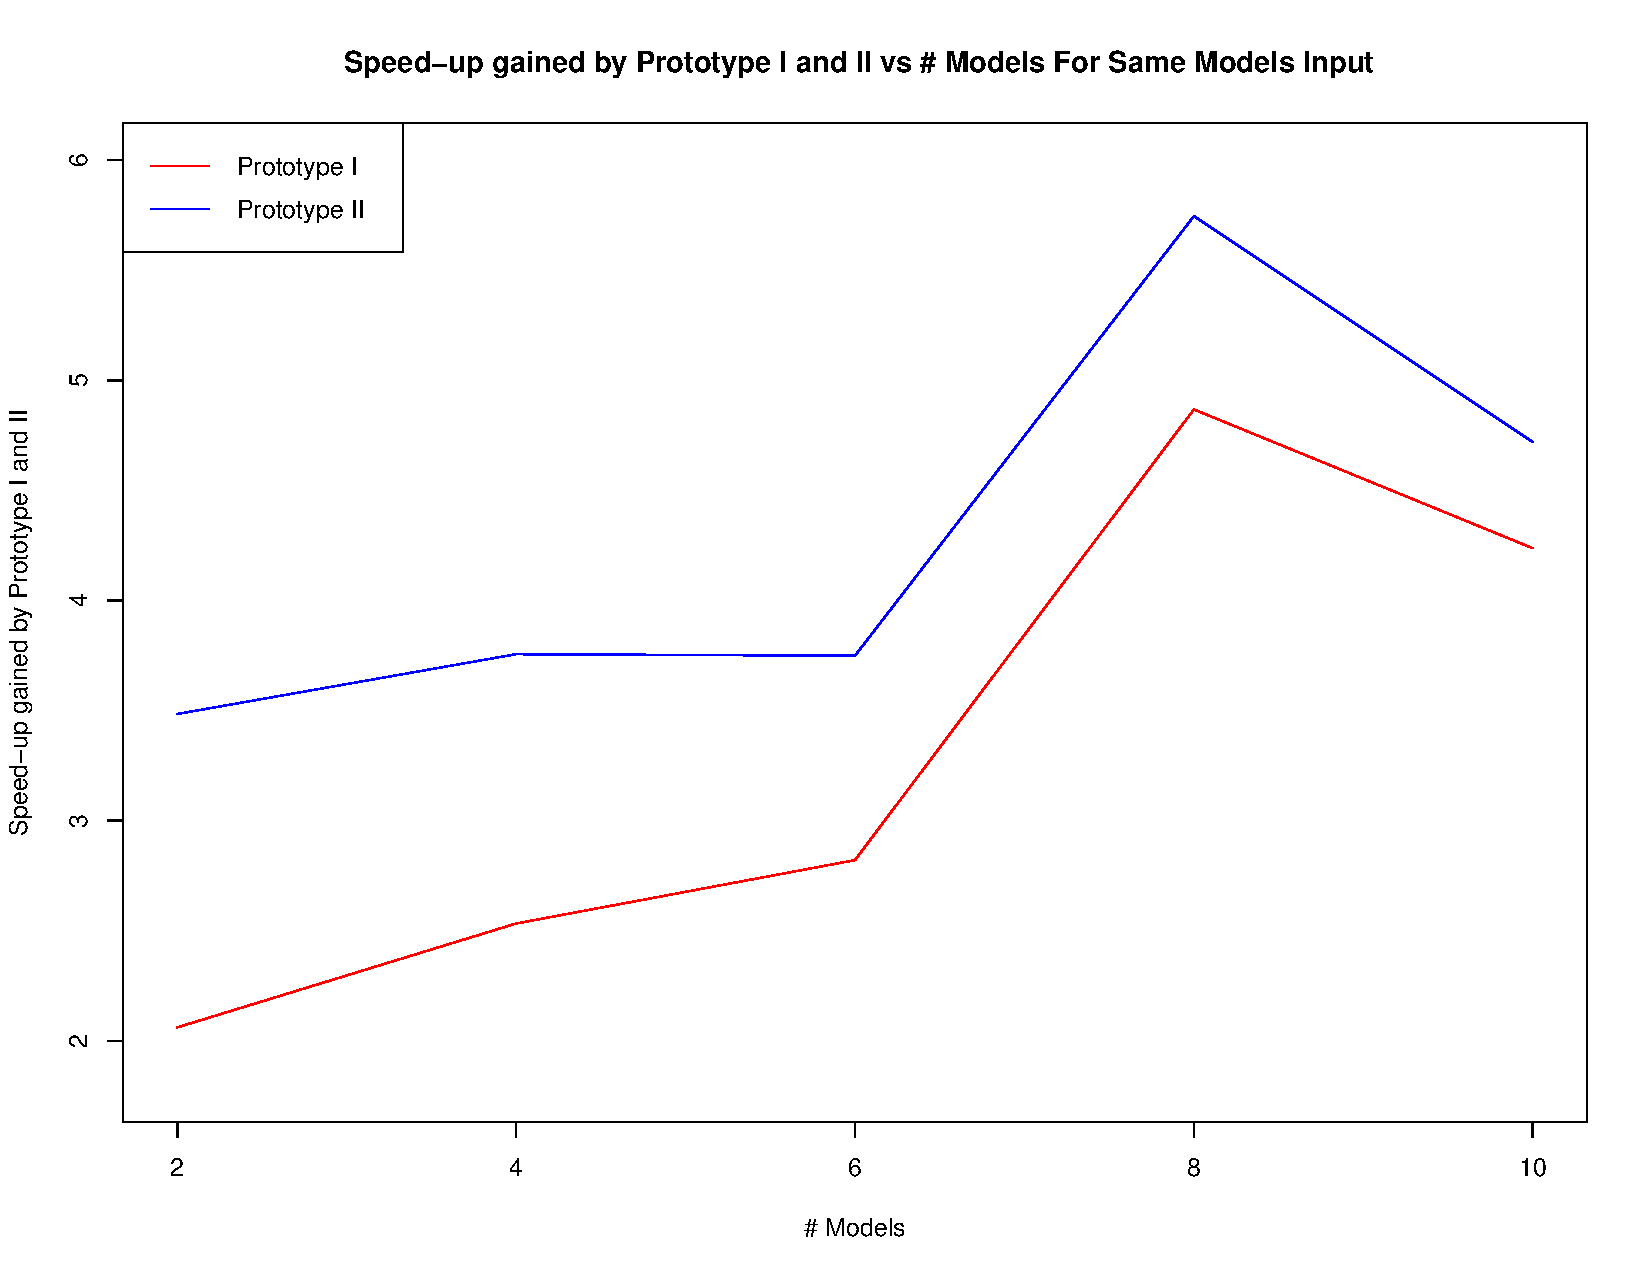
\includegraphics[width=0.9\textwidth]{SUPIPIIvsNumMod.pdf}
		\label{Fig:SUPIPIIvsNumMod}
\end{figure}
\end{frame}

\subsection{Prototype I vs Prototype II}
\begin{frame}
\begin{figure}[!ht]
		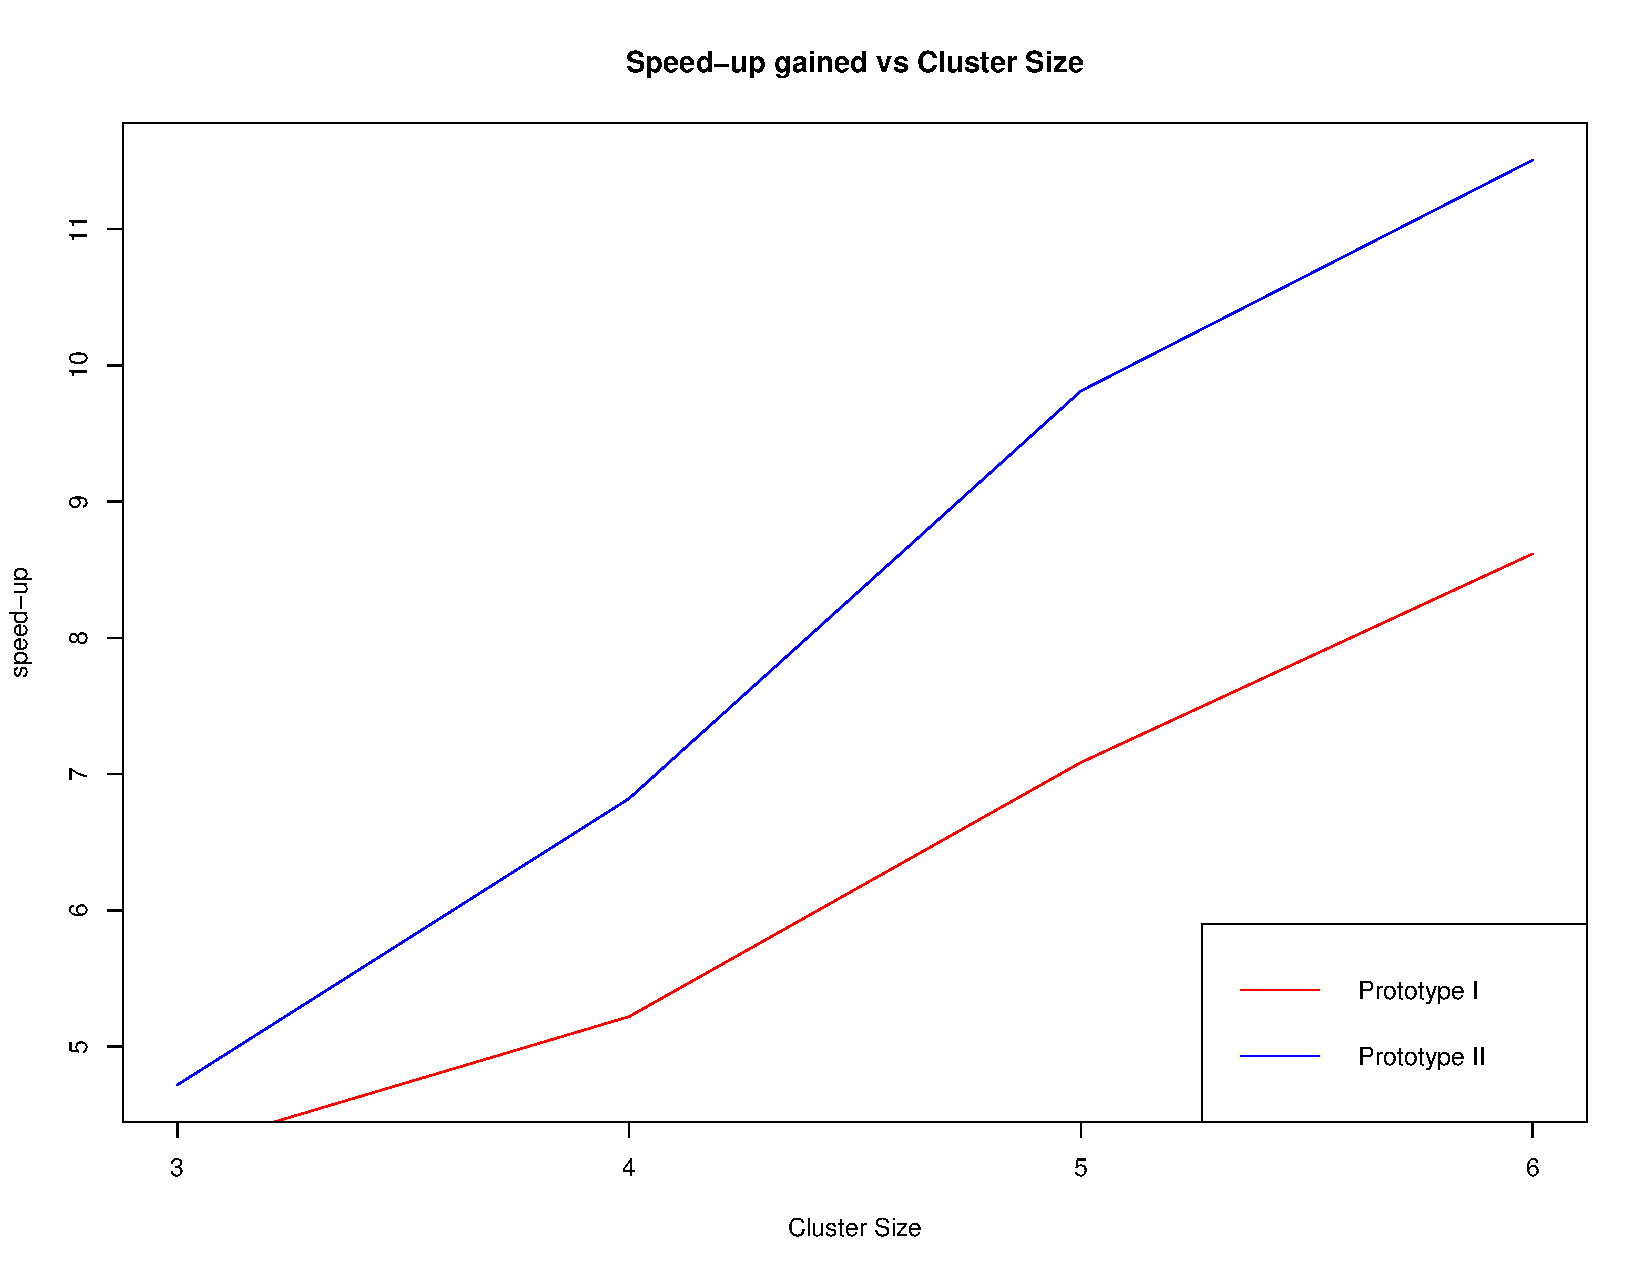
\includegraphics[width=0.9\textwidth]{SpeedupProtoIvsPrototII.pdf}
		\label{Fig:SpeedupProtoIvsPrototII}
\end{figure}
\end{frame}

\subsection{Prototype II Increase in Speed-Up}
\begin{frame}
\begin{figure}[!ht]
		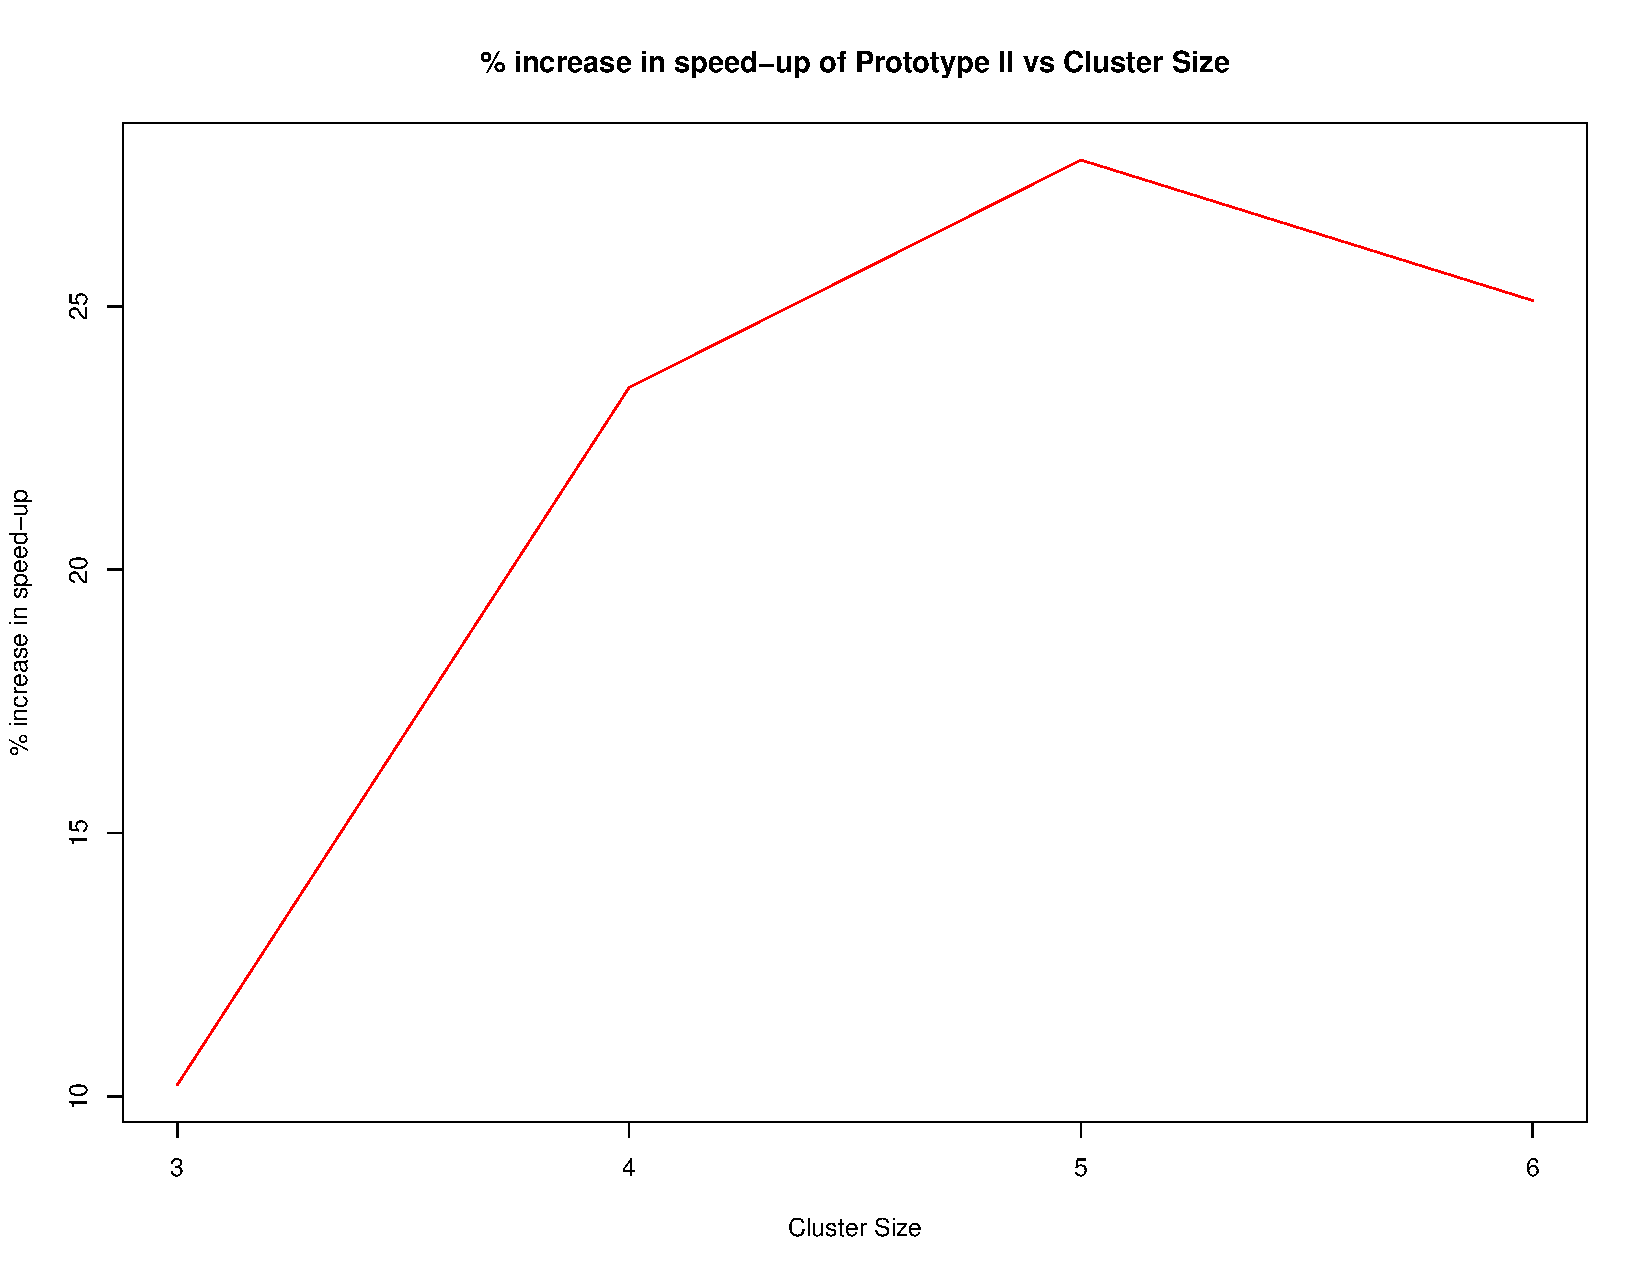
\includegraphics[width=0.9\textwidth]{IncSpeedUpProtoIIVsCS.pdf}
		\label{Fig:IncSpeedUpProtoIIVsCS}
\end{figure}
\end{frame}

\subsection{Profiling Prototype I}
\begin{frame}
\begin{figure}[!ht]
		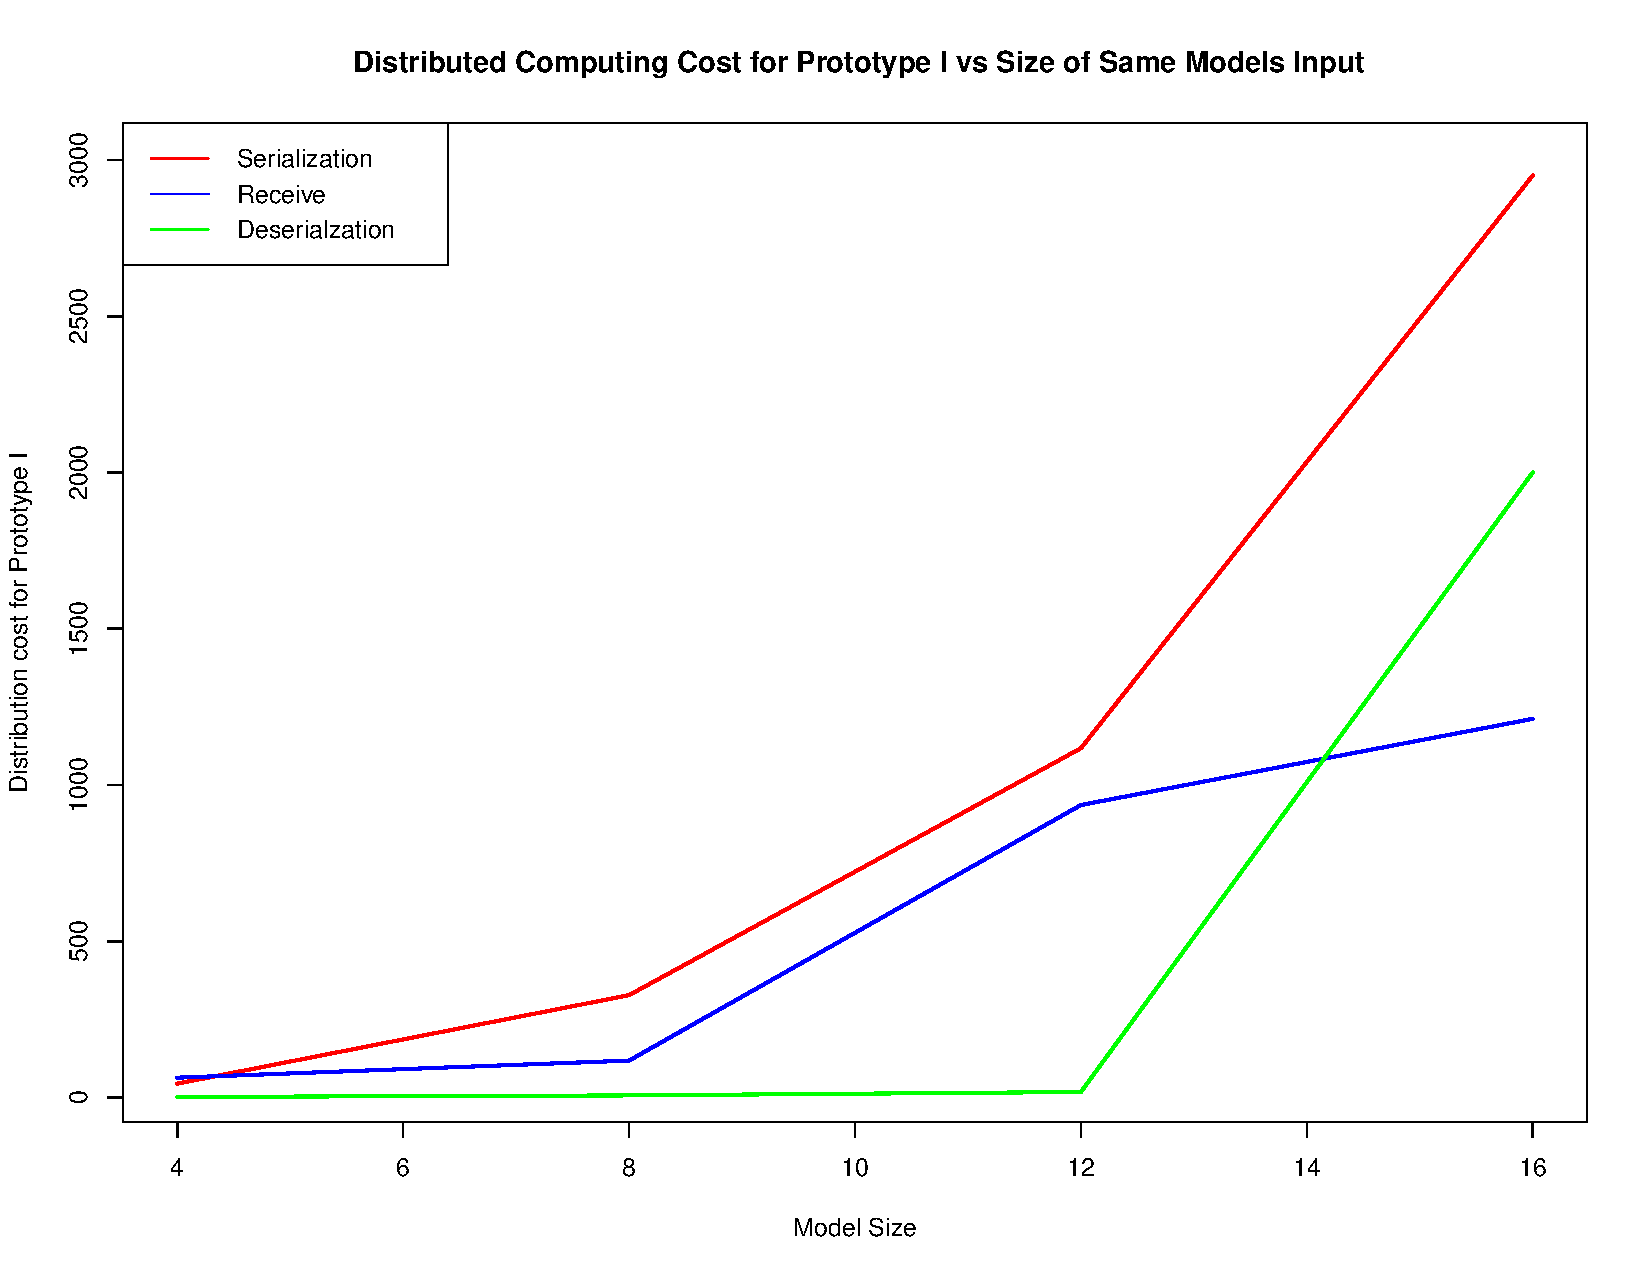
\includegraphics[width=0.9\textwidth]{DCPIvsCS.pdf}
		\label{Fig:DCPIvsCS}
\end{figure}
\end{frame}

\subsection{Profiling Prototype II}
\begin{frame}
\begin{figure}[!ht]
		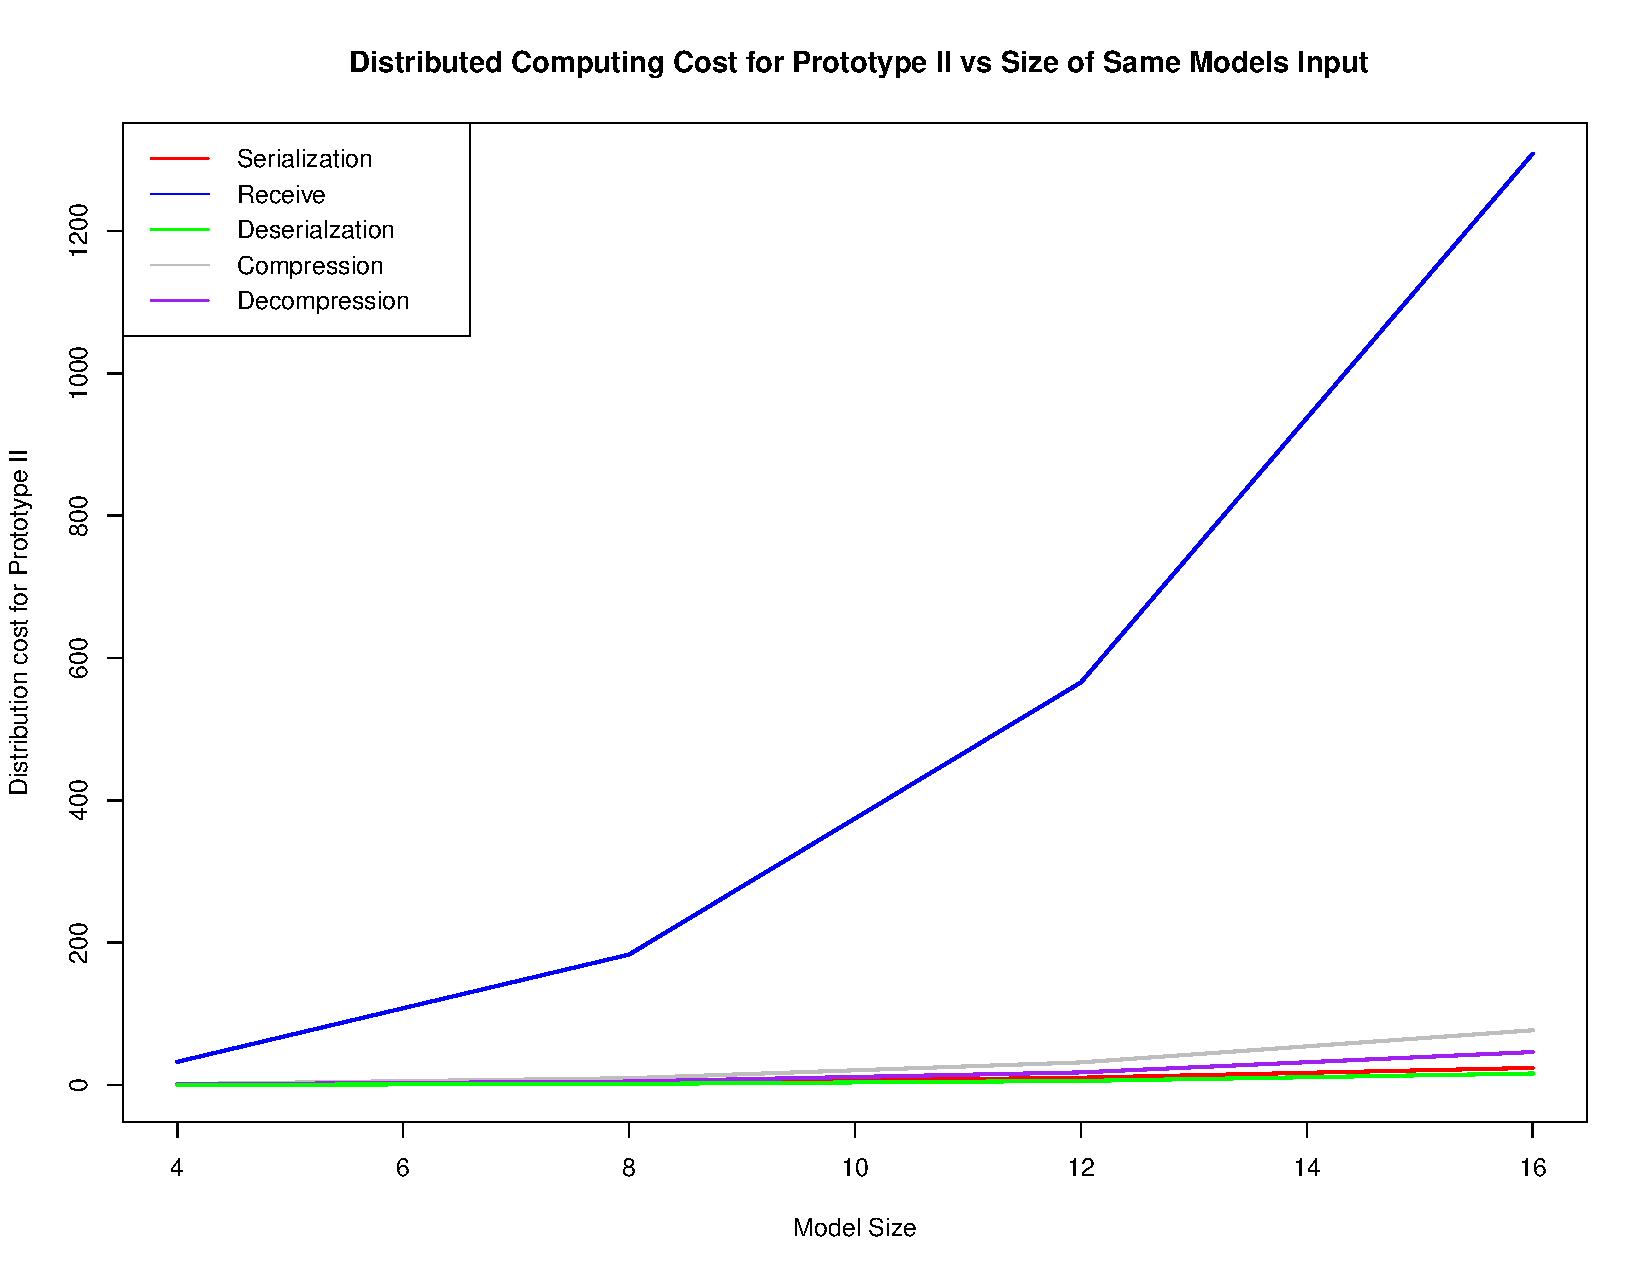
\includegraphics[width=0.9\textwidth]{DCPIIvsSize.pdf}
		\label{Fig:DCPIIvsSize}
\end{figure}
\end{frame}

\subsection{Prototype II: Design I vs Design II}
\begin{frame}
\begin{figure}[!ht]
		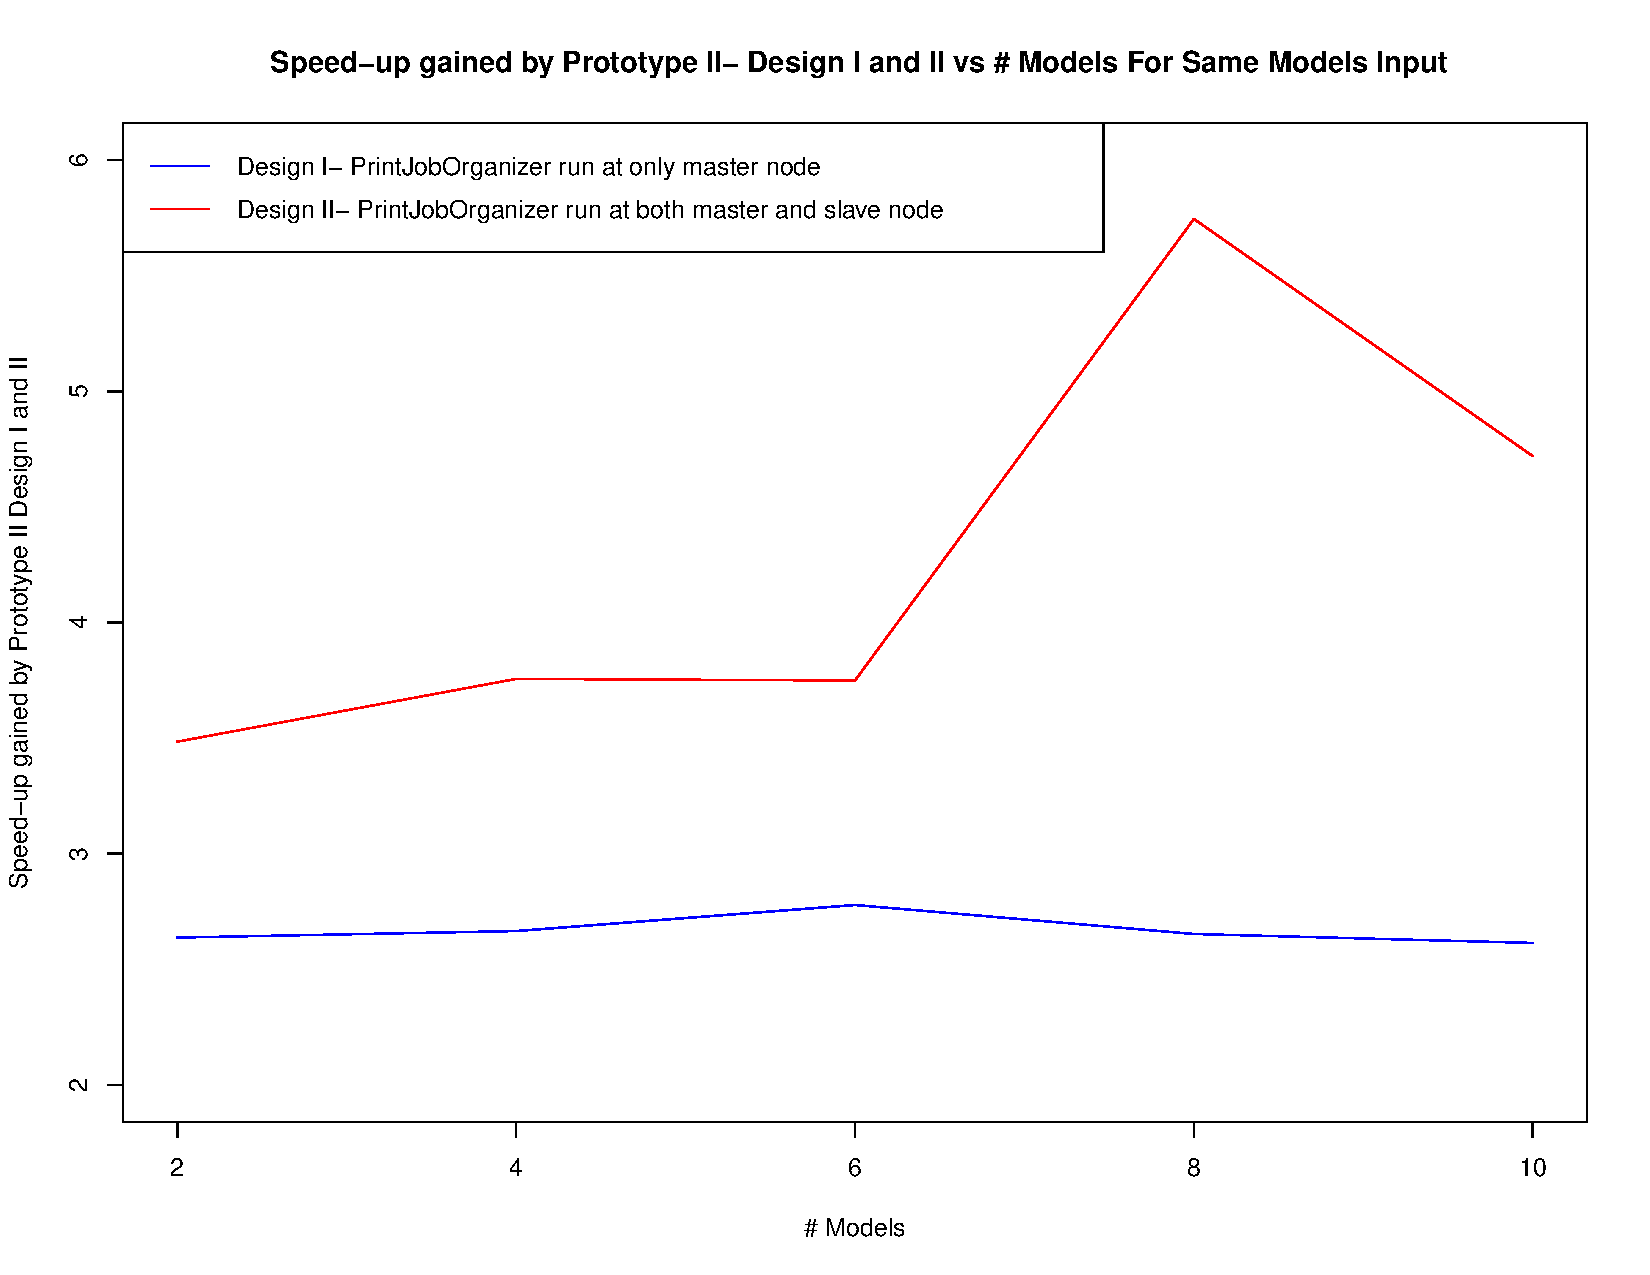
\includegraphics[width=0.9\textwidth]{SUDIDIIvsNumMod.pdf}
		\label{Fig:SUDIDIIvsNumMod}
\end{figure}
\end{frame}


\section*{Conclusion}
\begin{frame}
  \frametitle<presentation>{Conclusion}
	\begin{itemize}
	\item \textbf{Super-linear speed-up} can be achieved by distributed cuttlefish
	\item Prototype II has a better performance than Prototype I 
	\item Receive function might become a bottleneck for Prototype II 
	\item Disk I/O makes Prototype I slower 
	\item Composition of the Master and Slave Printing Software affects the Prototype II performance
\end{itemize} 
\end{frame}


\section*{Future Work}
\begin{frame}
  \frametitle<presentation>{Future Work}
	\begin{itemize}
	\item Develop new approaches for cost function calculation 
	\item Implementation of new communication mechanism 
		\begin{itemize}
		\item Replacing cluster computing with cloud computing
		\item Change in topology of the distributed system as well hardware acceleration
		\end{itemize} 
	\end{itemize} 
\end{frame}
\appendix
\section*{Appendix} 
\end{document}


